\documentclass{article}[12 pt]
\usepackage[utf8]{inputenc}
\usepackage[english]{babel}
\usepackage{tocloft}
\usepackage{lipsum}
\usepackage{sidecap}
\renewcommand\cftsecfont{\normalfont}
\renewcommand\cftsecpagefont{\normalfont}
\renewcommand{\cftsecleader}{\cftdotfill{\cftsecdotsep}}
\renewcommand\cftsecdotsep{\cftdot}
\renewcommand\cftsubsecdotsep{\cftdot}
\usepackage{graphicx}
\usepackage{hyperref,xcolor}

\definecolor{wine-stain}{rgb}{0.5,0,0}

\hypersetup
{
    colorlinks=true,
    linktoc = all,
    linkcolor = wine-stain,
    urlcolor = blue
}

\begin {document}

\title{Math Graphics README}
\author{Frank Basile, Janice Wallace, Daniel Etheridge}
\maketitle

\tableofcontents
	\section{Introduction}
		Math Graphics, is the final project for Group 12. The program is a fairly robust graphing calculator capable of displaying visual representations of mathematical functions on 2D Cartesian, 2D Polar, and 3D Cartesian graphs. Aside from displaying input functions, the calculator can also display derivatives and calculate definite integrals of single-variable functions in Cartesian 2D mode. Other features of the program include the ability to output the image of the graph to a file, as well as writing the independent and dependent variable data to a data format separated by any series of ASCII characters. Other features include the ability to customize the interface through the use of color changing palettes.

	\section{Installation}
	    No specific installation instructions are required. All that is required to run the program should be an updated version of Java and the executable file named MathGraphics.jar. For the latest version of Java, please check the \href{http://www.java.com}{Java homepage}.
	    
	\section{Starting the Program}
		Math Graphics has an easy to run interface. All that is required is to double click the MathGraphics.jar executable file. 
		
	\section{How To}
		\subsection{Initial Startup}
		When the program initially starts, the grapher is in Cartesian 2D mode and the function $sin(x)$ is displayed.:
			\begin{figure}[h!]
 				\centering
 				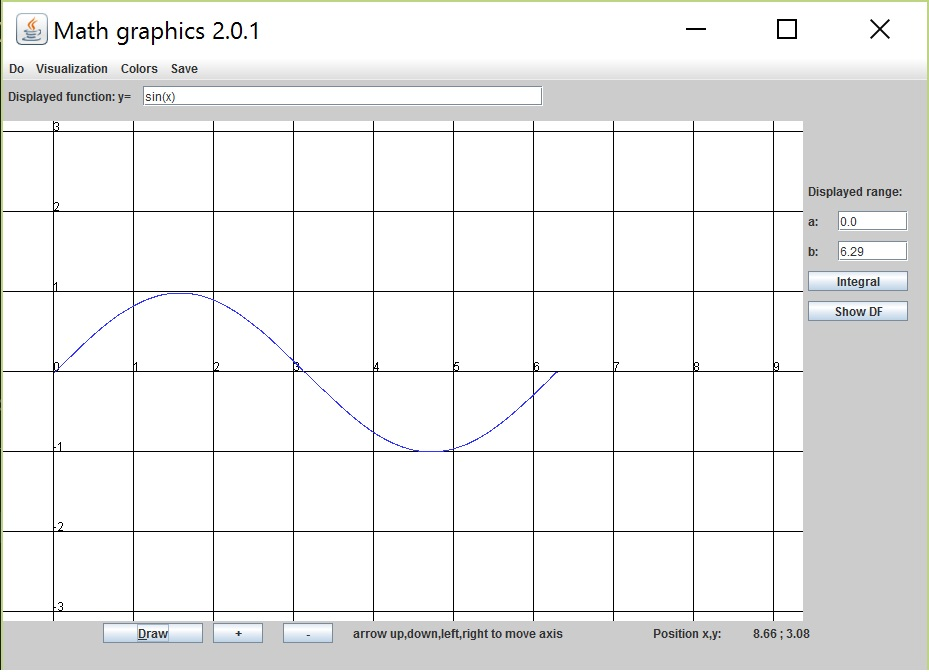
\includegraphics[scale = .75]{startupScreen}
 				\caption{The startup screen: $sin(x)$ is displayed}
 			\end{figure}
 		
 		\subsection{Basic Manipulation}
 		The Cartesian 2D screen offers a fairly robust number of options. These options include viewing the derivative of the function, changing the range of the displayed function,zooming in and zooming out on the graph, and an option to calculate the definite integral of the displayed function.  
 		
 			\subsubsection{View the Graph of the Derivative}
 			The derivative can be displayed by pressing the ``Show DF'' button. Alternatively, the derivative can be displayed from the drop down menu by clicking ``Do'' and ``Show DF.'' To hide the derivative simply press the ``No'' DF button. Or, from the drop down menu, select ``Do'' and ``No DF''.
 				\begin{figure}[h!]
 					\centering
 					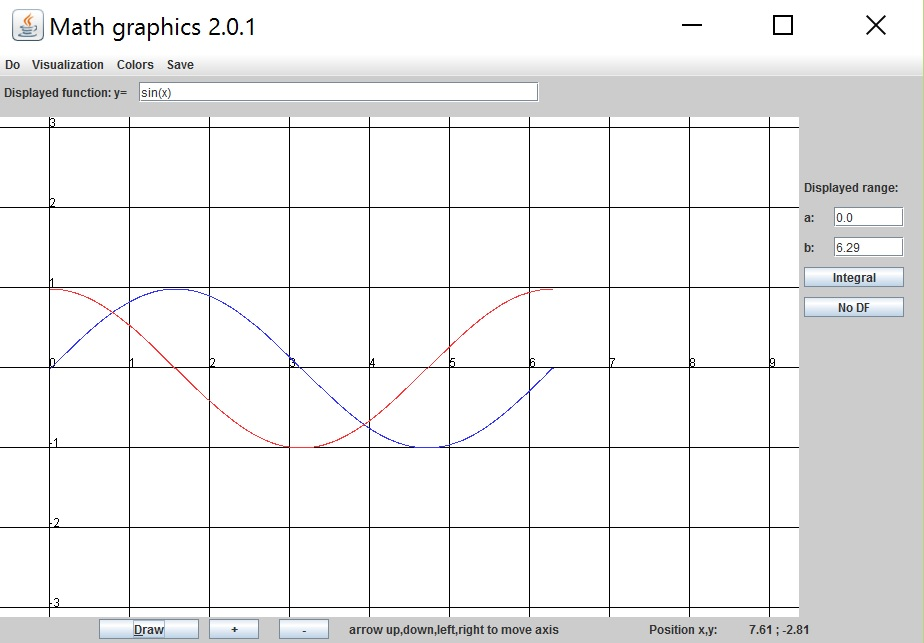
\includegraphics[scale = .75]{showDF}
					\caption{The derivative drawn after ``Show DF'' selected}
 				\end{figure}
				
			\subsubsection{Changing the Range of the Displayed Function}
 			Range changes can be made to the displayed function in Cartesian 2D mode. In order to do this, simply change the values of fields $a$ and $b$. Only valid numeric values can be input to these fields. It is not a requirement that $a < b$ as both the function and derivative can be drawn with $a < b$ or $a > b$.
 				
 			\subsubsection{Zoom Function}
			The graph can be zoomed in to specific points by clicking the ``+'' and ``-'' buttons located at the bottom of the screen. The graph will zoom in to the current center of the viewable graph. 

 		
 		\subsection{Changing the Displayed Function in 2D Modes}
 		\lipsum[1]
 				
\end {document}